% Copyright (c) 2021 Eclipse Arrowhead Project
%
% This program and the accompanying materials are made available under the
% terms of the Eclipse Public License 2.0 which is available at
% http://www.eclipse.org/legal/epl-2.0.
%
% SPDX-License-Identifier: EPL-2.0

The \GlossaryHyperRef{framework-arrowhead}{Arrowhead framework} itself consists of two categories of \GlossaryHyperRef{artifact}{artifacts}, as depicted in Figure \ref{fig:framework}.
The first category constitute a framework of assumptions, concepts, values and practices that frame the problem domain of \textit{dynamic device coordination in the context of automation}.
The second category it is a set of software specifications and \GlossaryHyperRef{implementation-software}{implementations} meant to address that problem domain.
In this section, we provide an overview of the primary \textit{concepts} of the Arrowhead framework.
While \textit{assumptions} and \textit{values} may be possible derive from this overview, no other framework artifacts are considered here or in the rest of this document.

\vspace*{1mm}

\begin{figure}[ht!]
  \centering
  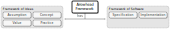
\includegraphics[scale=0.9]{figures/framework}
  \caption{
    The two main categories of artifacts of the arrowhead framework: ideas and software.
  }
  \label{fig:framework}
\end{figure}

\vspace*{-3mm}

\subsection{Stakeholders and Artifacts}

There are two kinds of members of the world of Arrowhead, (1) \GlossaryHyperRef{stakeholder}{stakeholders} and (2) \GlossaryHyperRef{artifact}{artifacts}, as depicted in Figure \ref{fig:world}.
The former denotes a person or organization engaged in an Arrowhead enterprise, while the latter is any thing or object, tangible or intangible, that could be relevant to consider as part of such an enterprise.
Stakeholders \GlossaryHyperRef{owner}{own}, \GlossaryHyperRef{supplier}{supply}, \GlossaryHyperRef{developer}{develop}, \GlossaryHyperRef{operator}{operate}, and \GlossaryHyperRef{user}{use} artifacts, among many other possible activities.
It is their business needs and ambitions that govern what and how Arrowhead artifacts will be employed.

\vfill

\begin{figure}[ht!]
  \centering
  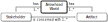
\includegraphics[scale=0.9]{figures/world}
  \caption{
    The two kinds of members of the Arrowhead world: stakeholders and artifacts.
  }
  \label{fig:world}
\end{figure}

\vspace*{-3mm}

\subsection{Devices, Systems and Services}

The most essential types of Arrowhead artifacts are (1) \GlossaryHyperRef{device}{devices}, (2) \GlossaryHyperRef{system}{systems} and (3) \GlossaryHyperRef{service}{services}, as shown in Figure \ref{fig:device-system-service}.
\textit{Devices} are physical machines with compute capabilities, making up the servers, robots, vehicles, tools, and other things part of the Arrowhead enterprise at hand.
Each device hosts, or runs, one or more \textit{systems}, which are \GlossaryHyperRef{communication}{communicating} \GlossaryHyperRef{instance-software}{software instances} that make their devices work toward whatever goals are set for them.
Finally, a \textit{service} is a set of related \GlossaryHyperRef{operation-service}{operations} that a system can make its device perform for a person or another system.
Services can be concerned with manufacturing, repair, analysis, or any other physical or virtual activity.
The service is the primary means whereby systems coordinate to fulfill their assignments.

\vfill

\begin{figure}[ht!]
  \centering
  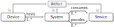
\includegraphics[scale=0.9]{figures/device-system-service}
  \caption{
    Hardware devices have, or \textit{host}, software systems, which \GlossaryHyperRef{provider-service}{provide} services.
    Each of these is an artifact.
  }
  \label{fig:device-system-service}
\end{figure}

\vspace*{-3mm}

\subsection{Service Provision and Consumption}

Communication between systems is formulated in terms of the \GlossaryHyperRef{provider-service}{provision} and \GlossaryHyperRef{consumer-service}{consumption} of services.
Systems may provide services, which other systems can consume by sending messages, as depicted in Figure \ref{fig:service-consumption}.

\begin{figure}[ht!]
  \centering
  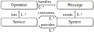
\includegraphics[scale=0.9]{figures/service-consumption}
  \caption{
    System consume services by sending message to them, which route them to the operations that concretely handle them.
    While not made explicit by this figure, sent and received messages move between systems and services by passing through \GlossaryHyperRef{interface}{interfaces}, as explained in Section \ref{sec:concepts:interface}.
  }
  \label{fig:service-consumption}
\end{figure}

When a service receives a message from a consumer, it \GlossaryHyperRef{routing-message}{routes} it to the specific operation it targets.
The operation will then handle the message by performing whatever activity it describes, as long as the message is valid.
This handling may entail sending additional messages to other services, starting or stopping various kinds of automation routines, among many other possible examples.

\subsection{System Composition}

When certain systems consume each other's services, they form a \GlossaryHyperRef{system-of-systems}{system-of-systems}.
Such a system-of-systems is able to perform activities none of its constituent \GlossaryHyperRef{subsystem}{subsystems} could perform on its own.
Two kinds of system-of-systems have particular significance in the context of the Arrowhead framework.
These are (1) the \GlossaryHyperRef{cloud-local}{local cloud}, and (2) the \GlossaryHyperRef{system-of-local-clouds}{system-of-local-clouds}, both depicted in Figure \ref{fig:system-of-systems}.

\begin{figure}[ht!]
  \centering
  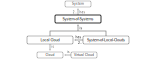
\includegraphics[scale=0.9]{figures/system-of-systems}
  \caption{
    The two primary kinds of Arrowhead systems-of-systems: the local cloud and the system-of-local-clouds.
  }
  \label{fig:system-of-systems}
\end{figure}

A \textit{local cloud} is a set of systems engaged in some form of physical activity that makes those systems physically bound to a particular location.
Local clouds come in many shapes and forms.
They may be completely stationary, completely mobile, or consist of both stationary and mobile devices.
Smelting stations, drone command centers, assembly lines, power distribution centers and satellite systems are a few examples of possible local clouds.

A \textit{system-of-local-clouds} is a set of local clouds, each kept distinct from the other local clouds by some form of boundary.
Boundaries may be organizational, physical, security-related, and so on.
Every system-of-local-clouds contains at least one local cloud that depends on another local cloud to perform some activity of relevance.
A systems-of-local-clouds could be formed by a set of weather stations, the robots of some collaborating parties at a mining site, the various departments of a manufacturing plant, and so on.
